\newpage
\section{eMoflon's graph viewer}
\genHeader

At this point, you should now have a small instance model. While Eclipse's built-in editor offers a nice tree structure and table to view and edit your model,
wouldn't it be nice to have a visualisation? eMoflon offers a ``Graph View'' to do exactly that! You'll find that this is an effective
feature to view how each element in your instance model interacts with others.

\begin{itemize}

\item[$\blacktriangleright$] When you first opened the eMoflon perspective, a small window to the right should have appeared with two tabs, ``Outline'' and
``Graph View.'' \footnote{If this window is not open, you can re-activate it by right-clicking on the ``eMoflon'' perspective in the main toolbar and pressing
``Reset,'' or by going to ``Window/Show View/Other..,'' then ``Other/Graph View''} 

\item[$\blacktriangleright$] Activate the second tab and drag one of your \texttt{Partition} instances into the empty window. 

\item[$\blacktriangleright$] To the right you can see the partition that was dragged in, visualised with all its immediate children
(Fig.~\ref{eclipse:graphView_init}).

\vspace{0.5cm}

\begin{figure}[htbp]
	\centering
  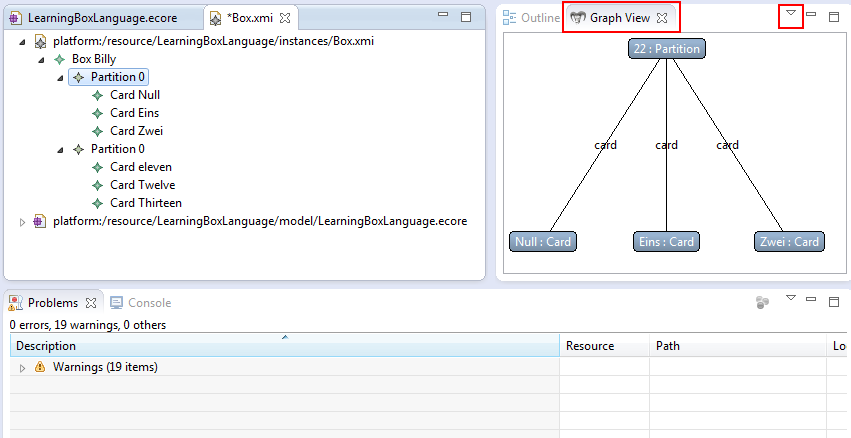
\includegraphics[width=1.0\textwidth]{eclipse_graphViewInit}
	\caption{A single partition in eMoflon's graph view}
	\label{eclipse:graphView_init}
\end{figure}

\vspace{0.5cm}

\item[$\blacktriangleright$] Clicking any item in the view will highlight it, and hovering over a node will list all its properties in a pop-up dialogue. If you
hover over a card, for example, you should be able to see their \texttt{back} and \texttt{face} values. You can also reposition elements.

\clearpage

\item[$\blacktriangleright$] Try dragging a second \texttt{Partition} element from the model to the viewer. As you can see, it doesn't replace the current
view, it simply places them side-by-side, showing the references between them partitions. To clear the screen, click the upside-down triangle in the top
right corner of the window, and select ``Clear View'' (Fig.~\ref{eclipse:graphView_init}).

\item[$\blacktriangleright$] To make the graph bigger, increase the size of the window, then select ``Redraw Graph'' from the same upside-down arrow. As you can
see, when an instance is already loaded, the graph view is not automatically updated. This option is useful if you change a property of an element (ie., the
\texttt{back} value of a \texttt{Card}) and wish to see it reflected in the graph.

\item[$\blacktriangleright$] Try experimenting with each of the different instance elements, viewer layouts and zoom settings found under the arrow. You'll
notice for the ``Spring Layout'' that each time you press ``Redraw Graph,'' the graph will re-arrange itself, even if you haven't updated any values or changed the window size.

\item[$\blacktriangleright$] The ``Graph View'' features is not exclusively for instance models; Expand the second root node in the editor, and drag and
drop the \texttt{LearningBoxLanguage} package into the viewer. Your entire metamodel is now completely displayed in the viewer
(Fig.~\ref{eclipse:graphView_typeGraph}). We have found that the ``Radial Layout'' works best for a view of this complexity. This might be confusing at first,
but the view contains your metamodel displayed in its abstract syntax, i.e., as an instance of Ecore. In contrast, the tree view displays the metamodel in UML-like
concrete syntax.

\vspace{1cm}

\begin{figure}[htbp]
	\centering
  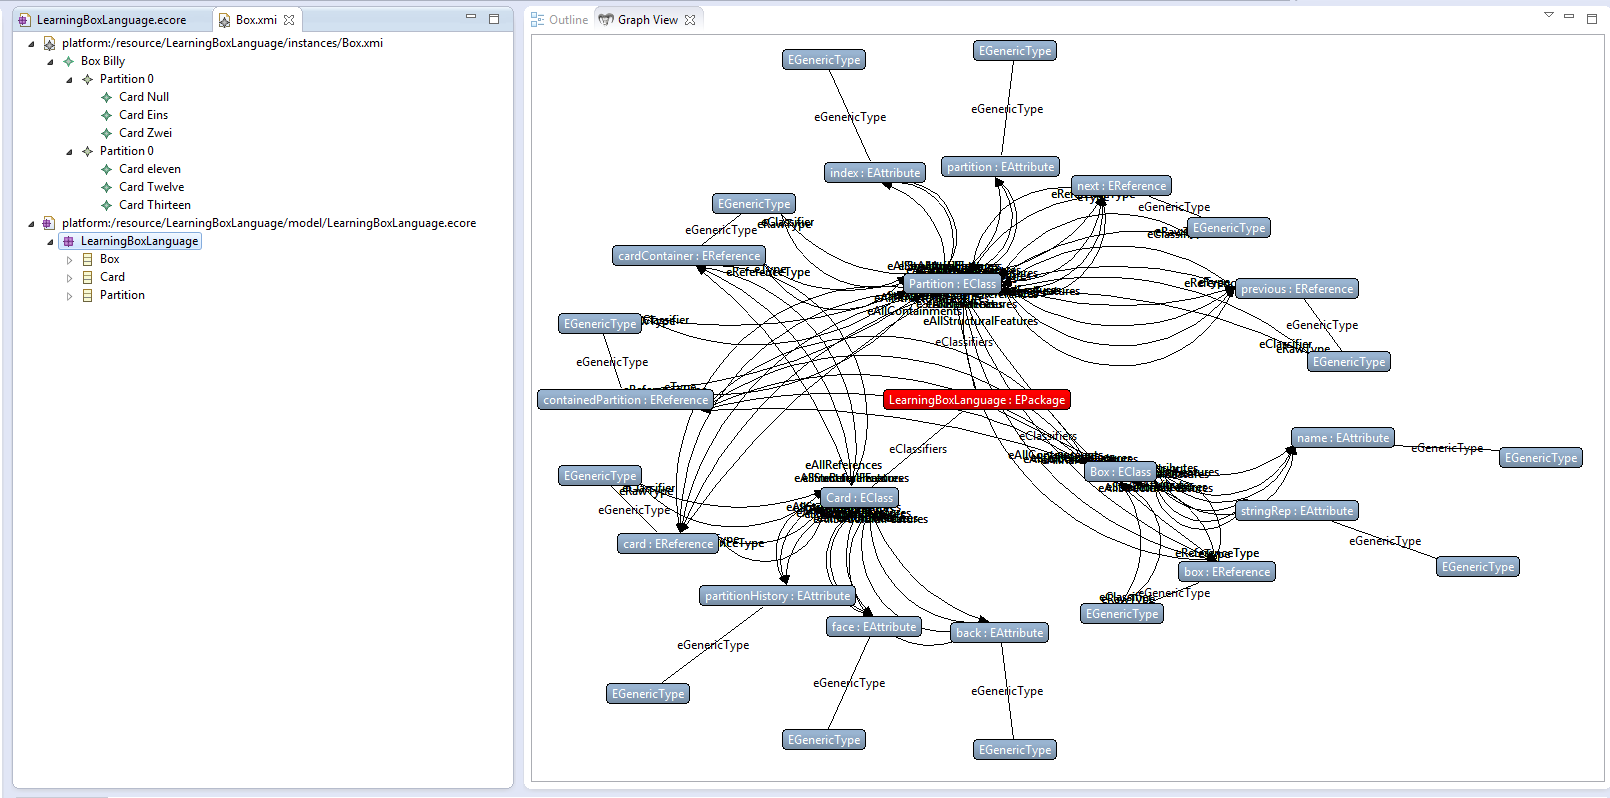
\includegraphics[width=0.9\textwidth]{eclipse_entireTypeGraph}
	\caption{Our instance's complete type graph}
	\label{eclipse:graphView_typeGraph}
\end{figure}


\end{itemize}
